\documentclass{article}
\usepackage{proof}
\usepackage{bussproofs}
\usepackage{xcolor}
\usepackage{url}
\usepackage{framed}
\usepackage{amsmath, amsfonts, amssymb}
\usepackage{mathtools}
\usepackage{minted}
\usepackage{stmaryrd}
\usepackage{verbatim}
\usepackage{graphicx}
\usepackage{hyperref}

\hypersetup{
	pdfborder={0 0 0},
	colorlinks=true,
	linkcolor=blue,
	urlcolor=blue,
	citecolor=blue
}
\usepackage{cleveref}


\newcommand{\rem}[1]{\textcolor{red}{[#1]}}
\newcommand{\ed}[1]{\textcolor{blue}{#1}}
\newcommand{\ct}[1]{\rem{#1 --ct}}

\begin{document}
	\title{Comprehensive Exam Report 2 - Relating Higher Order and First-Order Logics}
	\author{Arjun Viswanathan}
	\date{}
	\maketitle
	
	\section{Introduction}
	\label{sec:intro}
	In this report, we will discuss the 
	integration of automatic theorem provers 
	(ATPs) with interactive theorem 
	provers (ITPs). We will particularly
	focus on the ATP category of 
	satisfiability modulo theories (SMT) 
	solvers. ITPs are highly 
	reliable tools with a small proof kernel. 
	They require the user to write elaborate 
	proofs to formalize properties, and 
	provide little automation. ATPs, on the 
	other hand automatically prove formulas
	without any user intervention.  
	Users would benefit from having 
	the reliability of ITP results 
	with the automation capabilities
	of ATPs. However, SMT solvers have an 
	enormous code base, and due to the 
	lack of a small, verifiable kernel, 
	are susceptible to bugs. Thus, in a 
	collaboration with an SMT 
	solver, an ITP's trust-base would be 
	extended to include the solver's. To 
	avoid compromising the proof kernel of 
	the ITP, SMT solvers can 
	produce proofs of their results. 
	We explore how proof producing 
	SMT solvers can guide ITPs in 
	finding proofs for formulas - 
	a process called \textit{proof 
	search}. To assist ITPs in automation
	of proof search, the proof object from 
	the SMT solver guides the proof search 
	in the ITP via a process called
	\textit{proof reconstruction}.
	Reconstruction can be implemented 
	as a meta-procedure. For example, 
	reconstruction of SMT solver proofs 
	in Isabelle/HOL are done external to 
	the prover's logic~\cite{bohme}.
	Here, the external ATP's proof guides 
	\textit{Metis}, Sledgehammer's
	internal ATP in its proof search.
	The final proof is found by 
	\textit{Metis} and the SMT solver's 
	proof is only used to prune the 
	search space, and fill in holes.
	In SMTCoq~\cite{DBLP:phd/hal/Keller13},
	this reconstruction is 
	expressed within the ITP's logic 
	by a process called 
	\textit{computational reflection}.
	Here, the SMT solver's logic is 
	embedded in Coq's logic, and then 
	a proof from the SMT solver is 
	directly used to obtain the 
	proof of a formula in Coq. 
	While this reduces the 
	proof obligation within Coq, it incurs
	an overhead of checking the SMT 
	solver's proof, which is typically 
	large, inside Coq, making it a
	potentially time consuming process. 
	We look in detail into both these 
	approaches of integrating SMT solvers 
	with ITPs.
	
	\section{Preliminaries}
	\label{sec:prelims}
	
	In both Coq and Isabelle/HOL,
	lists are constructed using 
	square brackets (\texttt{[ ]})
	and their elements are separated 
	using semicolons (\texttt{;}). 
	Arrays are constructed using 
	curly braces (\texttt{\{ \}})
	and their elements separated 
	using commas (\texttt{,}).
	
	Declarative rules of the form
	\begin{center}
		$\infer[rule\_name]{C}{P_1 & ... & P_n}$
	\end{center}
	specify that if the premises $P_1$ to 
	$P_n$ hold, then the conclusion $C$
	holds.
	
	\subsection{Many-Sorted First-Order Logic}
	\label{sec:msfol}
	Many-sorted first-order logic extends
	first-order logic (FOL) with 
	types or sorts. We present the 
	syntax in this section and the 
	semantics are presented in
	\cite{Barrett2018}. Syntactically, 
	the components of MSFOL are sorts 
	$\sigma$, terms $t$, and 
	formulas $\phi$. Sorts are 
	atomic entities that 
	represent types. Function types 
	--- ($\sigma_1$, ..., $\sigma_n$) 
	$\to$ $\sigma$ ---
	and relation types 
	--- ($\sigma_1$, ..., $\sigma_m$)
	are defined over sorts, and 
	are types of functions and 
	predicates below. Terms $t$ and 
	formulas $\phi$ are specified as:
	\begin{align*}
	t &:= x^{\sigma}\ |\ 
	f^{(\sigma_1, ..., \sigma_n) \to 
		\sigma}	(t_1, ..., t_n)\\
	\phi &:= \bot\ |\ \neg \phi\ |\ 
	\phi_1 \land \phi_2\ |\ \forall 
	x^{\sigma} . \phi\ |\ t_1 = t_2
	\ |\ P^{\sigma_1,...,\sigma_m}
	(t_1, ..., t_m)
	\end{align*}
	Terms are either sorted variables, 
	or applications of functions to terms.
	Formulas are constants or logical 
	connectives applied to other 
	formulas, quantified formulas, 
	equality over terms, or predicates 
	over terms. Connectives $\lor$, 
	$\to$, $\leftrightarrow$, and the 
	existential	quantifier $\exists$ 
	can be specified using the connectives 
	and quantifiers mentioned above.
	
	A \textit{literal} is a term, or a 
	formula with no connectives other than 
	$\neg$. A \textit{clause} is a 
	disjunction of literals. All formulas 
	can be converted to conjunction normal 
	form (CNF) which is a conjunction of 
	clauses. For ease of notation, 
	a formula in CNF is also represented
	as a set of clauses within curly 
	braces. $\bot$, the formula 
	representing Boolean false, 
	is overloaded to also represent
	the empty clause, which is trivially
	unsatisfiable (unlike the empty set,
	or the empty conjunction which is 
	trivially satisfiable).
	
	The resolution rule simplifies two 
	clauses to a new clause as follows:
	\begin{center}
		$\infer[resolution]{\phi_1 \lor ... \lor 
			\phi_n \lor \psi_1 \lor ... \lor 
			\psi_m}{\phi_1 \lor ... \lor \phi_n 
			\lor \chi & \neg \chi \lor \psi_1 
			\lor ... \lor \psi_m}$ 
	\end{center}
	The following is an instance of the 
	resolution rule.
	\begin{center}
		$\infer{a \lor c}{a \lor \neg b 
			& b \lor c}$
	\end{center}
	Given that two clauses (a clause 
	is a disjunction of literals) hold, 
	and a \textit{pivot}, which is a 
	literal that occurs with opposite 
	polarities in each clause ($b$ in 
	the above example), the resolution 
	rule concludes that 
	the combination of the two clauses 
	without either occurrence of the 
	pivot holds.
	
	\subsection{Higher-Order Logic}
	\label{sec:hol}
	We specify the 
	syntax of higher-order logic 
	and delegate the explanation of 
	semantics to a 
	reference~\cite{10.5555/155278}. 
	HOL consists of 
	types $\tau$ and terms $t$. 
	\begin{align*}
	\tau &:= \alpha\ |\ \kappa^n\ 
	\tau_1 ... \tau_n\\
	t &:= x^{\tau}\ |\ c^{\tau}\ |\ t_1\ t_2\ 
	|\ \lambda x^{\tau}.t
	\end{align*}	
	Types $\tau$ are either type
	variables $\alpha$ or 
	applications of type 
	constructors $\kappa^n$ to 
	$n$ types ($n$ is usually omitted). 
	Particular types of interest are 
	the function type --- formed by 
	applying the arrow type constructor 
	$\to^{2}$ to other types, the 
	Boolean type --- $\texttt{Bool}$ 
	(or $\texttt{Bool}^0$), the type of 
	natural numbers --- \texttt{Nat},
	and integers --- \texttt{Int}.
	Note that $\texttt{Bool}$ is the 
	type of Booleans in higher-order
	logic (used only in 
	Sec.~\ref{sec:hammer}), different
	from \texttt{bool} which is the 
	type of Booleans in Coq (used only 
	in Sec.~\ref{sec:smtcoq}).
	Terms are typed variables, 
	typed constants, applications 
	of terms to terms, or typed
	$\lambda-$ abstractions. We have
	the usual Boolean constants 
	representing logical connectives
	and quantifiers. For instance, 
	logical negation, 
	$\neg^{\texttt{bool} \to 
		\texttt{bool}}$, universal 
	quantification,
	$\forall^{\alpha \to 
		\texttt{bool} \to \texttt{bool}}$, 
	and polymorphic equality,
	$=^{\alpha \to \alpha 
		\to \texttt{bool}}$. Type 
	annotations for terms are also 
	often omitted when understood
	from context.
	
	
	\section{SMTCoq}
	\label{sec:smtcoq}
	SMTCoq is a skeptical cooperation 
	between the Coq proof assistant, and 
	SAT and SMT solvers, implemented as a 
	Coq plugin. We will maintain a focus 
	on the SMT solver integration of 
	SMTCoq, noting that most features are 
	shared with the SAT	solver integration.
	
	\begin{figure}
		\begin{framed}
			\textsc{Step 1}: Coq calls SMTCoq over 
			a Boolean formula $F$:
			\begin{minted}{Coq}
Theorem F : forall (a b c : bool), (b && negb c) || 
  (a && negb b) || negb a || c = true.
Proof.
  smt.
			\end{minted}
		\end{framed}
		
		\begin{center}
			$\big\downarrow$
		\end{center}
		
		\begin{framed}
			\begin{center}
				\textsc{Step 2}: SMT solver 
				proves $F$ and returns proof 
				\texttt{t}. This step is 
				expanded in Fig.~\ref{fig:smtex}
			\end{center}
		\end{framed}
		
		\begin{center}
			$\big\downarrow$
		\end{center}
		
		\begin{framed}
			\textsc{Step 3}: SMT Coq's checker 
			checks deep embedding of $F$, 
			\texttt{f}, against proof 
			\texttt{t}:
			\begin{center}
				\texttt{checker f t = true}
			\end{center}
		\end{framed}
		
		\begin{center}
			$\big\downarrow$
		\end{center}
		
		\begin{framed}
			\textsc{Step 4}: Reflection principle 
			reflects deep embedding to shallow 
			embedding $\mathbb{I}(\texttt{f})$:
			\begin{center}
				\texttt{checker\_correct f t 
					(refl\_equal (checker 
					f t) true)}
			\end{center}
		\end{framed}
		
		\begin{center}
			$\big\downarrow$
		\end{center}
		
		\begin{framed}
			\textsc{Step 5}: Proof of $F$ is 
			completed in Coq:
			\begin{minted}{Coq}
Theorem F : forall (a b c : bool), (b && negb c) || 
  (a && negb b) || negb a || c = true.
Proof.
  smt.
Qed.
			\end{minted}
		\end{framed}
		
		\caption{SMTCoq's journey in proving 
			example Boolean formula $F$}
		\label{fig:smtcoqex}
	\end{figure}
	
	ATPs like SMT solvers are susceptible 
	to bugs due to the large code-bases 
	used to support	their automation. 
	ITPs like Coq have a small trustable 
	proof kernel which would be 
	compromised if they were to trust
	external results. In a collaboration
	with SMT solvers, to avoid extending 
	Coq's trust-base, SMTCoq requires the 
	solvers to be proof-producing, and uses 
	Coq's computational capabilities 
	to lift their proofs up to Coq proofs, 
	in a process called computational 
	reflection. This is illustrated in 
	Fig.~\ref{fig:smtcoqex} using a 
	running example that is elaborated 
	in the rest of the section.
	
	\begin{figure}[t]
		\begin{framed}
			\textsc{Step 2.1}: $F$ is negated:
			\begin{align*}
			F&: (b \land \neg c) \lor 
			(a \land \neg b) \lor \neg a 
			\lor c\\
			\neg F&: \neg((b \land \neg c) 
			\lor (a \land \neg b) \lor \neg 
			a \lor c)
			\end{align*}
		\end{framed}
		
		\begin{center}
			$\big\downarrow$
		\end{center}
		
		\begin{framed}
			\textsc{Step 2.2}: $\neg F$ after CNF 
			conversion is checked for 
			unsatisfiability by the SMT solver:
			\begin{align*}
			&\{\neg b \lor c, \neg a \lor b,
			a, \neg c\}
			\end{align*}
		\end{framed}
		
		\begin{center}
			$\big\downarrow$
		\end{center}
		
		\begin{framed}
			\textsc{Step 2.3}: SMT solver produces 
			proof \texttt{t} of 
			unsatisfiability of $\neg F$ or of
			validity of $F$:
			\begin{prooftree}
				\AxiomC{$\neg c$}
				\AxiomC{$\neg b \lor c$}
				\AxiomC{$\neg a \lor b$}
				\BinaryInfC{$\neg a \lor c$}
				\AxiomC{$a$}
				\BinaryInfC{$c$}
				\BinaryInfC{$\bot$}
			\end{prooftree}
		\end{framed}
		
		\caption{The SMT Solver's role in 
			helping SMTCoq prove example 
			formula $F$.}
		\label{fig:smtex}
	\end{figure}
	
	SMT solvers refutationally prove 
	input formulas --- given a formula
	$F$, the solver proves that the 
	negation of $F$ ($\neg F$) is 
	unsatisfiable, which is equivalent
	to proving that $F$ is valid. 
	To do this, the SMT solve converts 
	$\neg F$ into conjunction or clausal 
	normal form (CNF) which is a 
	conjunction of clauses. It then uses 
	a combination of a SAT solver and 
	multiple theory	solvers to reduce 
	the set of input clauses to the 
	empty clause via resolution
	and other rules of inference. Thus,
	deriving the empty clause, which 
	represents the most trivial
	inconsistency in CNF, from the 
	input clauses proves that the input 
	clauses 
	are unsatisfiable. A proof
	from an SMT solver is a tree 
	with the input clauses (from the 
	negation of the input formula) at
	the leaves and $\bot$
	at the root. The role of the SMT
	solver from Fig.~\ref{fig:smtcoqex}
	is elaborated in Fig.~\ref{fig:smtex}.
	The SMT solver's proof creation is 
	detailed in Report 3.
	
	SMTCoq implements a checker for 
	SMT solver proofs (Step 3). It 
	encodes the language of SMT solvers
	in Coq as two different embeddings. 
	Given a logical framework A, and 
	a logical framework B, in which we 
	want to represent the language of A, 
	there are two ways to achieve this
	representation, and 
	both of these are necessary for 
	reflection:
	\begin{itemize}
		\item \textit{Shallow Embedding: }
		Use types and terms of B that 
		correspond to those of A, to 
		represent terms of A. A shallow
		embedding of SMT formulas in 
		Coq is Coq's \texttt{bool} 
		type of Booleans.
		\item\textit{Deep Embedding: }
		Define custom types in B that 
		correspond to those of A, and 
		define inside B, the meaning of 
		terms of these custom types with 
		respect to shallow terms. A 
		deep embedding of SMT formulas 
		is defined as the type 
		\texttt{form} in SMT solvers.
		\texttt{f} from 
		Fig.~\ref{fig:smtcoqex} has
		type \texttt{form}.
	\end{itemize}
	
	Given formula $F$, SMTCoq's proof 
	checker checks the deep embedding of 
	$F$ against the proof of $F$ from the 
	SMT solver. If the checker succeeds, 
	SMTCoq is able to reflect the formula in 
	the deep embedding to its shallow 
	embedding. This is done via a 
	correctness lemma for the checker
	(also called the reflection principle),
	which proves that for any 
	formula in the deep embedding, if 
	the checker is able to check an SMT
	proof against it, then the formula in 
	the shallow embedding is true. A 
	proof of $F$ in the shallow 
	embedding is obtained by instantiating 
	the correctness lemma with $F$.
	Step 4 from Fig.~\ref{fig:smtcoqex} 
	shows the instantiation of 
	the reflection principle with 
	the right objects to obtain the 
	proof of our example formula. 
	The interpretation function
	$\mathbb{I}$ transforms 
	formulas in the deep embedding
	to their shallow embeddings
	given a valuation $\nu$ of the 
	free variables, so 
	$\forall\ \nu,\ 
	\mathbb{I}_{\nu}(\texttt{f})$
	is exactly the proof required 
	to close theorem $\texttt{F}$
	in Coq. The reflection principle 
	is explained in Section~\ref{sec:refl}.	
	
	SMTCoq is \textit{sound} ---
	when it proves a formula in Coq, the 
	formula is valid and thus the proof
	can be closed (using \texttt{Qed.},
	as in Fig.~\ref{fig:smtcoqex}, 
	step 5), but 
	not \textit{complete} --- when it 
	fails to prove a formula, we can't 
	be certain that the formula isn't 
	valid. This is because, the underlying 
	SMT solver cannot decide certain 
	formulas - given a formula, it could 
	either return \texttt{sat} 
	(satisfiable), \texttt{unsat} 
	(unsatisfiable), or 
	\texttt{unknown} (`don't know').
	Additionally, SMTCoq only works for 
	quantifier-free SMT theories. The 
	theories it currently supports 
	are the theories of equality over
	uninterpreted functions (EUF), 
	liniear integer arithmetic (LIA),
	bit-vectors (BV), and arrays with
	extensionality (AX).
	
	\subsection{Checker}
	\label{sec:checker}
	SMTCoq's checker checks the deep embedding
	of SMT formulas in Coq against the 
	proof trees discharged by the SMT solver.
	Recall that a deep embedding is an
	inductive type written in 
	Coq representing SMT formulas. 
	In the following, we present 
	a simplified version of SMTCoq's 
	deep embedding. The actual embedding 
	uses Coq's machine integers to 
	implement sharing of terms and 
	optimize space, but an unoptimized 
	and simpler version is presented 
	below. 
	
	\texttt{form} is the type of 
	formulas:
	\begin{minted}{coq}
	Inductive form : Type :=
	| Fatom (_ : atom)
	| Ftrue
	| Ffalse
	| Fnot (_ : form)
	| Fand (_ : array form)
	| For (_ : array form)
	| Fimp (_ : array form)
	| Fxor (_ _ : form)
	| Fiff (_ _ : form)
	| Fite (_ _ _ : form)
	\end{minted}
	where a formula can be an atom, 
	\texttt{true}, \texttt{false};
	a negation of a formula; a 
	conjunction, disjunction, or 
	implication of any number of
	formulas; an exclusive-or or
	an equivalence of two formulas; 
	or, an if-then-else of three formulas.
	\texttt{atom} is the type of atoms
	or terms:
	\begin{minted}{Coq}
	Inductive atom : Type :=
	| AppIntr (_ : op) (_: list atom)
	| AppUnintr (_ : int) (_: list atom).	
	\end{minted} 
	which can be applications of 
	either interpreted functions 
	(from a theory) or uninterpreted
	functions to zero (constants) or more 
	terms. Uninterpreted functions 
	are parameterized by machine 
	integers while interpreted ones 
	are encoded as follows:
	\begin{minted}{Coq}
	Inductive op : Type :=
	| Zcst (_ : Z) | Zle | Zlt | Zplus | ...
	| Eq (_ : type).
	\end{minted}
	Some of the interpreted integer 
	functions are shown in \texttt{op}.
	Similarly, there are interpreted 
	functions from each theory.
	Some examples of atoms are 
	\begin{itemize}
		\item \texttt{AppUnintr 0 [AppUnintr 
			1 []]} for the term $f(x)$ where 
		$f$ has index $0$, and $x$ has 
		index $1$; 
		\item \texttt{AppIntr Zplus [(AppIntr 
			(Zcst 5) []); (AppUnintr 2 [])]} 
		for the term $5 + y$ where $y$ 
		has index $2$.
		\item Recursively, from the previous example,
		\texttt{AppUnintr
			1 []} for $x$.
		\item Recursively, from the previous example,
		\texttt{AppUnintr 2 []} for $y$.
	\end{itemize}
	Finally, for convenience of representing 
	CNF formulas in SMTCoq, a \texttt{clause} 
	data structure encodes a disjunction of 
	literals as a list of its constituents 
	and a \texttt{state} represents the entire 
	formula in CNF as an array of the 
	respective conjuncts. Thus, the deep 
	embedding of formula $F$ from our running 
	example, is the encoding of the set 
	$\{\neg b \lor c, \neg a \lor b, a, 
	\neg c\}$ from step 2.2 of 
	Fig.~\ref{fig:smtex} 
	as the following \texttt{state}:
	\begin{align*}
	\{&\texttt{[Fnot Fatom (AppUnintr 1 []); 
		Fatom (AppUnintr 2 [])],} &(*\ \neg b \lor c\ *)\\
	&\texttt{[Fnot Fatom (AppUnintr 0 []);
		Fatom (AppUnintr 1 [])],} &(*\ \neg a \lor b\ *)\\
	&\texttt{[Fatom (AppUnintr 0 [])],
		[Fnot Fatom (AppUnintr 2 [])]}\} &(*\ a, \neg c\ *)  
	\end{align*}
	where $a, b,$ and $c$ are indexed as 
	$0, 1,$ and $2$.
	
	The checker inputs a formula in its 
	deep embedding, and a proof of the 
	formula from the SMT solver, and 
	returns \texttt{true} if the proof 
	proves the formula, and 
	\texttt{false} otherwise:
	\begin{center}
		\texttt{checker : form 
			$\to$ T $\to$ bool}	
	\end{center}
	More specifically, given deep embedding 
	\texttt{f} of type \texttt{form}
	and proof object \texttt{t} of type 
	\texttt{T}, it checks whether \texttt{t} 
	from the SMT solver is a proof of  
	unsatisfiability of	\texttt{$\neg$f}, and 
	returns \texttt{true} if it is. 
	Although all SMT solvers (that 
	interface with SMTCoq) provide a
	refutation tree as a proof, as 
	illustrated in step 2.3 of 
	Fig.~\ref{fig:smtex},
	their proof formats vary. CVC4 uses 
	LFSC~\cite{DBLP:journals/fmsd/StumpORHT13}
	which is a meta-logic that allows the 
	specification of proof calculi that have 
	declarative	rules with computational 
	components called side conditions, and 
	veriT uses a proof language similar to 
	SMTLIB~\cite{Besson1}. SMTCoq has its 
	own proof certificate format for SMT 
	solver proofs and it translates proofs 
	from all solvers to this certificate 
	format, and \texttt{T} is the type of 
	these certificates that are 
	checked by the checker. Note 
	that these translators are outside 
	Coq's trusted kernel, but are kept
	small, and tested using a large 
	set of benchmarks. 
	
	\begin{figure}[t]
		\begin{center}
			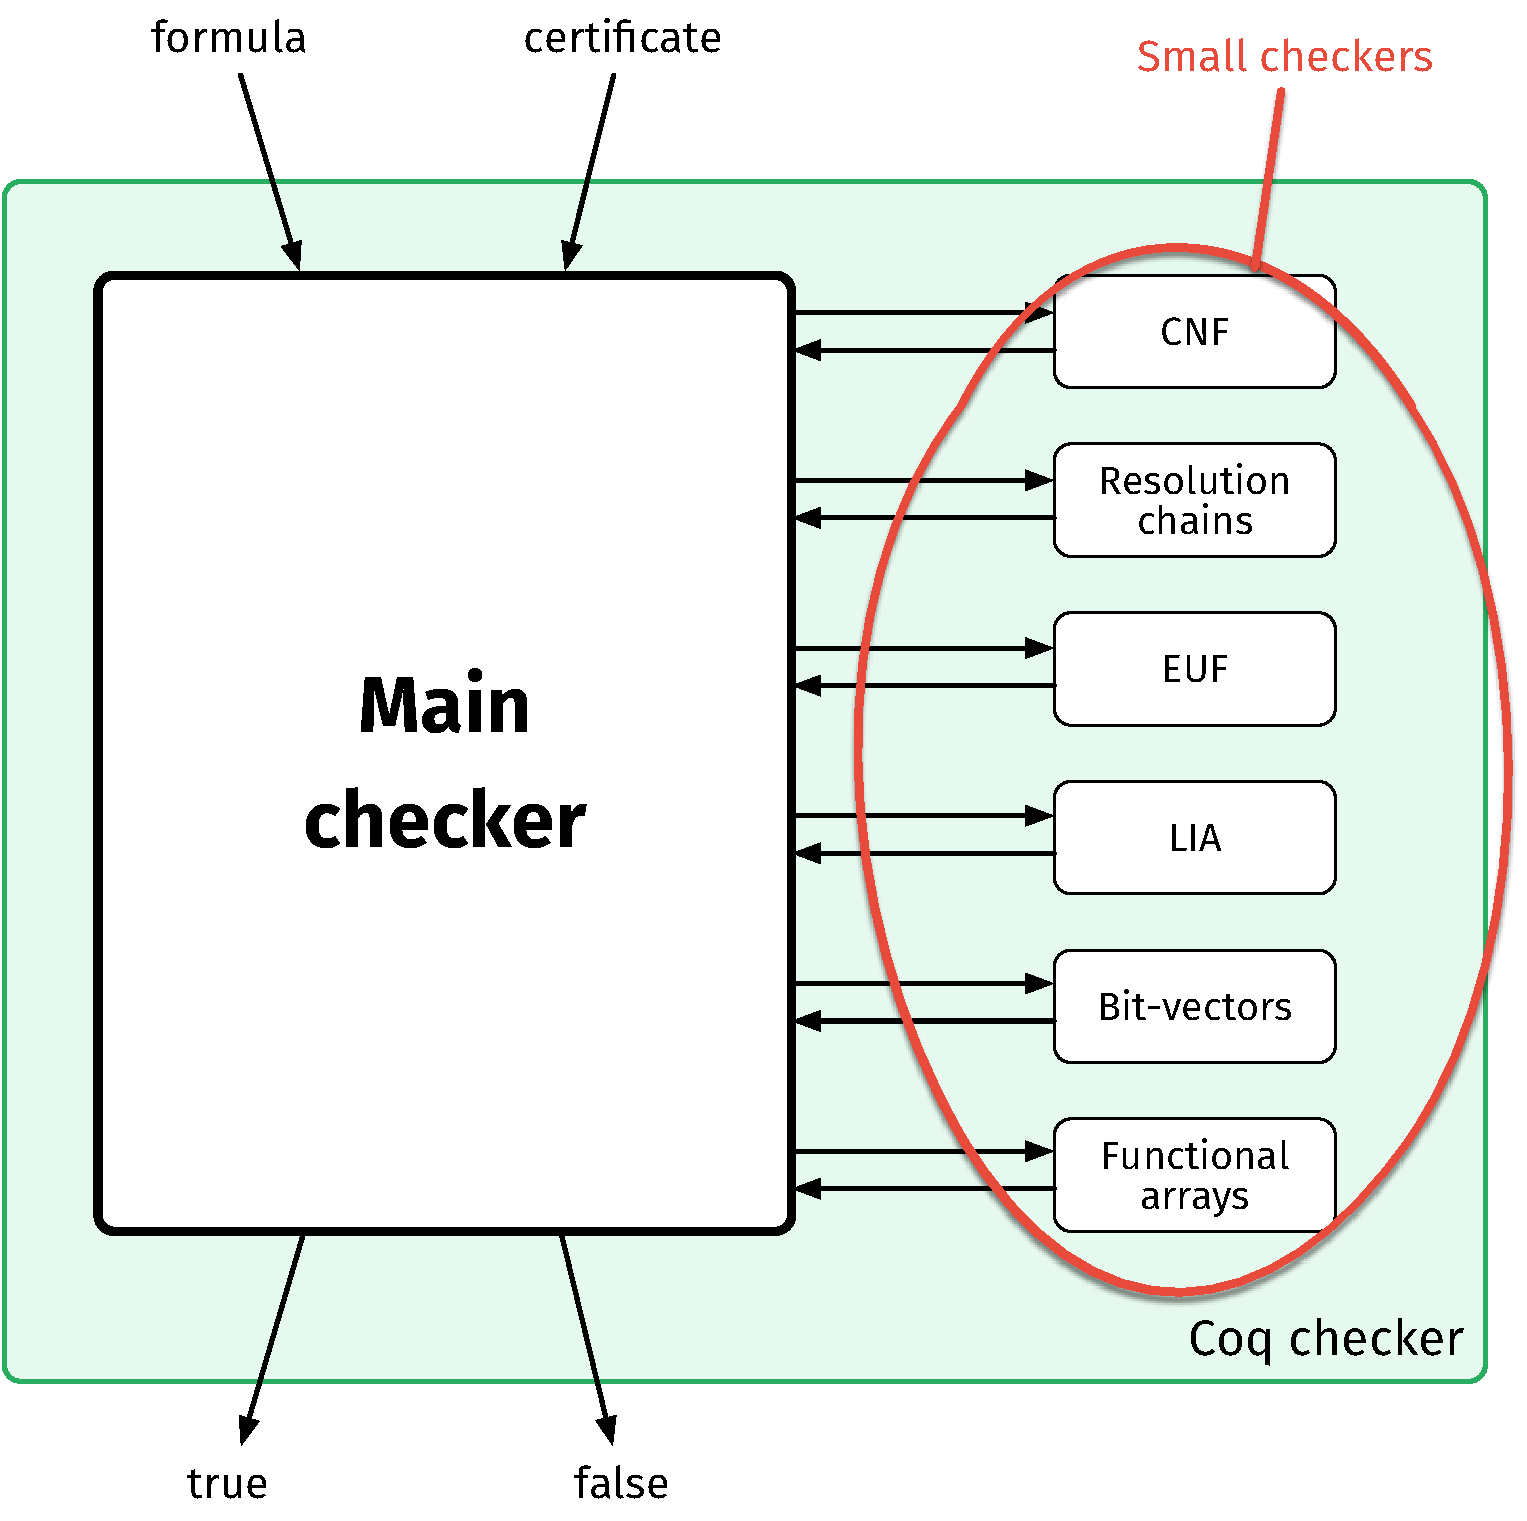
\includegraphics[scale=0.3]{checker}
			\caption{SMTCoq's \texttt{checker}
				shown as the "Main checker" which 
				interacts with various small checkers.}
			\label{fig:checker}
		\end{center}
	\end{figure}
	
	To prove the unsatisfiability of a 
	formula, the SMT solver operates in 
	phases. It converts the formula into
	CNF and performs some simplications
	on it. It then abstracts any theory
	literals into propositional ones 
	and tries to satisfy the abstraction 
	using the SAT solver; it does this
	in a cycle where the theory
	solvers give feedback
	by adding the negation of the 
	satisfying model to the 
	abstraction of the formula, if the 
	refinement of the model isn't 
	satisfied in a theory. 
	Each of these phases constitute
	\textit{steps} of the SMT proof
	that SMTCoq has to check. A step
	can modify the current 
	\texttt{state} (representation of 
	the formula) while maintaining 
	its (un)satisfiability. If the 
	initial formula is unsatisfiable, 
	then after running all steps,
	the final \texttt{state} is the 
	empty clause $\bot$. Currently, 
	SMTCoq has steps that perform 
	resolution, conversion of formulas 
	to conjunction normal form (CNF), SMT 
	solver simplifications, and one for 
	each theory. Each step is 
	independently checked by a small 
	checker. Each small
	checker simplifies the  
	\texttt{state} via the step it 
	performs, and the main checker 
	(\texttt{checker}) ultimately checks 
	that the input is 
	finally transformed to $\bot$. The 
	architecture of the checker is 
	illustrated in
	Fig.~\ref{fig:checker}. The phases 
	of SMT solver operation and the 
	corresponding steps of the
	SMT solver's proof are elaborated
	in Report 3.
	
	\subsection{Reflection Lemma}
	\label{sec:refl}
	The previous section describes a 
	deep embedding of SMT formulas 
	in Coq and a checker for 
	proofs of these formulas (step 3 of 
	the running example in 
	Fig.~\ref{fig:smtcoqex}). 
	This infrastructure alone serves 
	as an external checker for 
	SMT solver proofs in Coq.
	SMTCoq, however, is able to 
	do more than this, as demonstrated
	in steps 4 and 5. In addition 
	to checking SMT solver proofs, 
	it can lift these up to 
	Boolean formulas in Coq and
	prove such formulas automatically
	in Coq with the assistance of 
	the SMT solver. In principle,
	this is done by proving the
	correctness of \texttt{checker}
	with respect to \texttt{Bool}
	formulas, that is to say that 
	for every formula (\texttt{form})
	that \texttt{checker} is able to 
	successfully check against its
	proof from the SMT solver, the 
	corresponding \texttt{Bool}
	formula holds. The entities
	that these deep embeddings 
	must correspond to are the shallow
	embeddings, and the correspondence 
	itself is defined by the 
	interpretation function. The 
	shallow embedding, interpretation
	function, and the correctness 
	lemma are discussed in this 
	section.
	
	The shallow embedding of SMT formulas
	have Coq's \texttt{Bool} type of 
	Booleans. The advantage of a 
	shallow embedding in a logical 
	framework is that it is usually 
	a subset of the framework's language
	and doesn't need to be defined. 
	As in the deep embedding, Boolean
	formulas may have atoms containing 
	terms from the theories of 
	equality, integers, bit-vectors,
	and arrays. Boolean equality and
	the Coq $\mathbb{Z}$~\cite{CoqZ} type 
	of integers are sufficient to encode
	the first two, while SMTCoq 
	defines custom types for 
	bit-vectors and arrays. The
	respective shallow embeddings of
	the examples used to illustrate 
	the deep embedding of atoms in the 
	previous section are simply 
	\texttt{f(x)} and \texttt{5 + y} 
	with \texttt{f, x,} and \texttt{y}
	correctly typed. The shallow 
	embedding for our running example 
	is the formula from the lemma we 
	are trying to prove in Coq
	(Step 1 of fig.~\ref{fig:smtcoqex}):
	\begin{center}
		\texttt{(b \&\& negb c) || (a 
			\&\& negb b) || negb a || c}
	\end{center}	 
	SMTCoq deals only with an effectively 
	quantifier-free fragment of the SMT 
	solver's logic. Even though quantifiers 
	appear in the theorem in Coq (Step 1 of 
	Fig.~\ref{fig:smtcoqex}), because
	of the structure of universal 
	quantification where all the variables
	are quantified only in the beginning 
	of the formula and the scope of 
	each quantifier is the entire formula, 
	it is straightforward
	to instantiate away the quantifiers
	using the \texttt{intros} tactic, which 
	only leaves the quantifier-free 
	formula in the proof context, and this 
	is exactly what SMTCoq does. 
	Thus, it suffices to consider the 
	unquantified version of the 
	formula from the example.
	
	The interpretation function 
	has the following type.
	\begin{center}
		$\mathbb{I} :\ \texttt{form} \to 
		\texttt{val} \to \texttt{bool}$
	\end{center}
	Given a \texttt{form} \texttt{f} 
	and a valuation $\nu$ of free 
	variables in \texttt{f}, the 
	interpretation function returns 
	the shallow embedding of \texttt{f}
	with the variables in \texttt{f} 
	assigned values as specified by 
	$\nu$. The interpretation of a 
	formula \texttt{f} for a valuation 
	$\nu$ is represented as $\mathbb{I}_{\nu}
	(\texttt{f})$. 
	
	Finally, the 
	\textit{reflection principle}, 
	or the reflection lemma, is a 
	lemma proving the checker correct
	in terms of the shallow embedding.
	\begin{align*}
	\texttt{checker\_correct} :\ 
	\forall\ \texttt{(f : form)
		(t : T) checker f t = true} \to \\
	\forall\ (\nu : \texttt{val}),\ 
	\mathbb{I}_{\nu}(\texttt{f}) = 
	\texttt{true}
	\end{align*}
	If a checker is able to check 
	some formula \texttt{f} in 
	the deep embedding against
	some proof certificate \texttt{t} from 
	the SMT solver (it checks that 
	\texttt{t} proves the unsatisfiability
	of \texttt{$\neg$f}), then 
	\texttt{checker\_correct},
	proves that the shallow embedding,
	or the interpretation of \texttt{f}
	holds for any valuation of the 
	variables in \texttt{f} (thus 
	proving it valid). 
	
	It is called the reflection 
	principle, because it uses 
	computational reflection 
	to shift the burden of the 
	proof to a computation --- 
	the computation done by 
	the checker. Since 
	\texttt{checker\_correct}
	is proved for all formulas 
	and certificates, it can be 
	instantiated with any 
	particular formula and 
	certificate. The only thing it 
	requires, to 
	prove the interpretation of 
	the formula, is that the checker
	returns \texttt{true}.
	Since SMT solver proofs are 
	often large, this is a 
	heavy computation. The
	reflection mechanism reduces
	proving to computations via 
	Coq's reduction mechanism.
	Coq's Calculus of Inductive 
	Constructions (CIC) is a 
	$\lambda-$calculus that has a 
	reduction mechanism for terms. The
	reduction rules form a strongly 
	normalizing system. The calculus's
	\textit{conversion rule} allows a 
	term to have multiple types, as long as 
	the types have the same normal forms. 
	For instance, for some predicate $P$ 
	over natural numbers, a term that 
	has type $P(10)$ also has type 
	$P(5*2)$ and $P(20-10)$. Due 
	to the conversion rule, 
	computations can be used in Coq's 
	reasoning and proof terms can be 
	found simply by computing normal 
	forms of types.
	
	Returning to our running example, 
	step 4 of 
	Fig.~\ref{fig:smtcoqex} illustrates
	a call to the reflection principle by
	SMTCoq. Given 
	deep embedding \texttt{f}
	of the formula in the example, and 
	SMT proof certificate \texttt{t} of 
	\texttt{f}, the proof of $\forall\ \nu,\ 
	\mathbb{I}_{\nu}(\texttt{f}) = 
	\texttt{true}$ is simply:
	\begin{center}
		$\texttt{checker\_correct f t
			(refl\_equal (checker f t) true)}$
	\end{center}
	where \texttt{refl\_equal} 
	(reflexivity of equality) is a tactic
	that forces the Coq type checker to 
	perform an equality check between 
	\texttt{checker f t} and 
	\texttt{true} by reduction. 
	The claim is that the two 
	terms are convertible to each other
	and since \texttt{true} is a simple 
	term of type \texttt{Bool}, 
	Coq's reduction mechanism is 
	invoked on \texttt{checker f t},
	which usually consists of checking
	a large non-trivial SMT certificate. 
	SMTCoq uses various optimizations 
	to make these computations efficient.
	As alluded to in the previous section,
	the deep embedding presented there 
	only conceptually resembles SMTCoq's
	deep embedding. The implementation 
	of SMTCoq uses a non-recursive 
	structure with hash-consing of terms
	and machine integers to store variables,
	among other optimization tricks.
	Similar optimizations are also 
	applied to certificates.
	Since the reflection principle is 
	proved for general formulas, 
	each invocation of it only varies
	in the deep embedding and proof 
	certificate that it is instantiated
	with. This is a simple instantiation
	proof in Coq, the overhead
	being in reducing the call to 
	\texttt{checker} for each 
	formula and proof pairing to 
	\texttt{true}.
	
	The checker divides certificates
	into steps that can independently 
	checked by small checkers.
	Similarly, the correctness lemma
	of the checker also depends on 
	the correctness lemma of each 
	small checker. Recall that 
	small checkers modify the 
	\texttt{state} via steps that 
	they perform and eventually
	reduce the state to $\bot$ if 
	the certificate indeed proves
	unsatisfiability.  Thus, the 
	correctness lemma of a small 
	checker guarantees that it
	performs sound steps - that is,
	the step doesn't change the 
	satisfiability or unsatisfiability
	of the state. With these proofs
	of correctness from the step 
	checkers, if the steps do 
	convert the input formula 
	to $\bot$, then it is 
	straightforward for 
	\texttt{checker}
	to conclude that the 
	(negation of the) input is 
	unsatisfiable. The division 
	of a proof into steps and 
	the division of the main 
	checker into checkers for these
	steps contribute to a 
	modular architecture where it 
	is fairly straightforward to 
	add new steps (like new theories)
	to SMTCoq without breaking 
	the rest of the system --- one 
	needs to extend the step type,
	write a checker for the step, 
	and prove it correct. The 
	certificate format for SMT
	proofs also makes it 
	convenient to integrate a 
	new SMT solver with SMTCoq, 
	no matter what its proof format
	--- one need only write a translator
	from the proof format of the SMT
	solver to the certificate format. 
	As a testament to the utility of
	SMTCoq's modularity, it's 
	initial iteration had veriT as 
	the only SMT solver integrated, 
	and EUF and LIA as the only 
	theories. It was extended 
	with support for CVC4 and 
	for the theories of 
	bit-vectors and 
	arrays~\cite{DBLP:journals/corr/EkiciKKMRT16}.
	
	
	\section{Sledgehammer}
	\label{sec:hammer}
	Isabelle~\cite{DBLP:journals/corr/cs-LO-9301106} 
	is an LCF-style system that 
	provides a meta-logic which can be 
	instantiated with other logics.
	Isabelle/HOL~\cite{10.5555/1791547}, 
	one of the most popular Isabelle 
	instantiations, implements a 
	classical higher-order logic. 
	
	Sledgehammer is
	an Isabelle/HOL component that 
	uses external ATPs to enhance 
	Isabelle/HOL with proof 
	automation. Initially, these 
	ATPs only included resolution 
	provers~\cite{10.1007/978-3-642-39799-8_1}.
	The work by Bohme et 
	al.~\cite{bohme} involved 
	extending Sledgehammer to 
	incorporate SMT
	solvers~\cite{Barrett2018} and this 
	work will be our focus for the 
	rest of this section. As with 
	SMTCoq, the SMT solvers integrated
	with Sledgehammer produce a 
	proof object which is 
	then reconstructed within
	Isabelle/HOL by Sledgehammer, 
	using Sledgehammer's own internal 
	ATP --- Metis~\cite{hurd2003d}. The 
	proof object essentially guides 
	the inference steps of the proof 
	within Isabelle/HOL.
	
	\begin{figure}[t]
		\begin{center}
			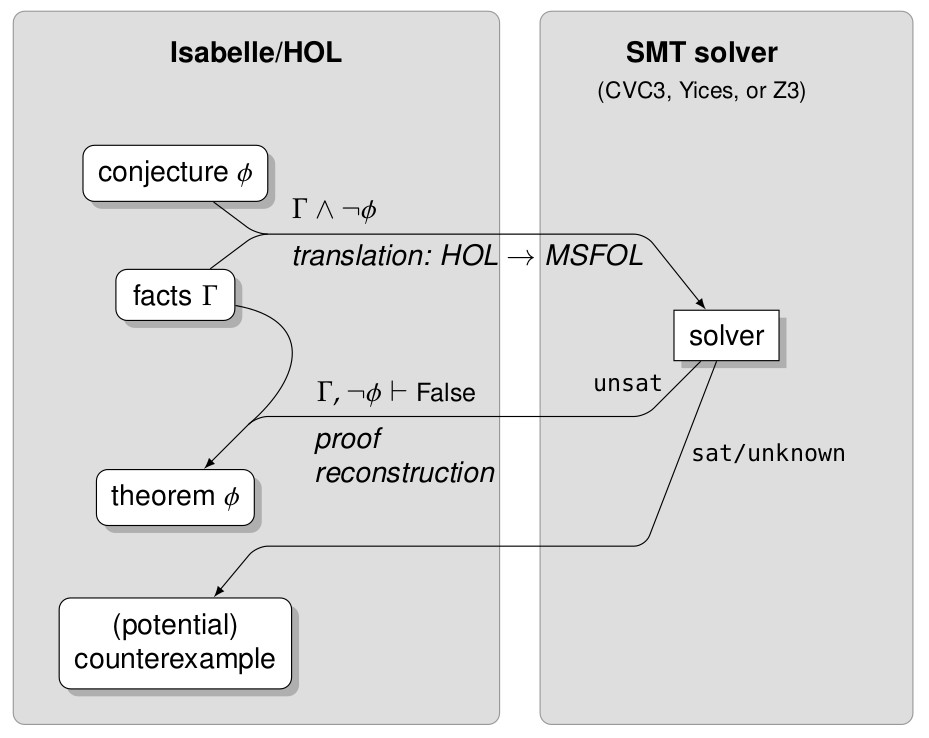
\includegraphics[scale=0.3]{sledgehammer}
			\caption{SMT solvers' integration with 
			Isabelle/HOL}
			\label{fig:sledgehammer}
		\end{center}
	\end{figure}

	The integration of Sledgehammer 
	with SMT solvers is illustrated in 
	Fig.~\ref{fig:sledgehammer}. Given 
	a conjecture $\Phi$ in 
	Isabelle/HOL, Sledgehammer 
	selects a set of facts 
	$\Gamma$ that might be relevant 
	to proving $\Phi$ and sends
	the formula $\Gamma \land \neg 
	\Phi$ to the SMT solver to check 
	for unsatisfiability. If the SMT 
	solver finds the formula to be 
	satisfiable, it returns a satisfying 
	model, which serves as a 
	counterexample 
	of the conjecture. If the SMT 
	solver is able to refute the 
	conjecture (i.e., conclude 
	the unsatisfiability of its 
	negation), it returns 
	a proof. The proof tree (that
	proves $\bot$ from the 
	input) is then reconstructed in 
	Isabelle/HOL via a bottom-up 
	traversal of the tree, where 
	for each node, a theorem is 
	added to Isabelle/HOL by Metis.
	Unlike SMTCoq, this reconstruction
	process occurs external to 
	Isabelle/HOL's logic ---
	an external procedure guides 
	the reconstruction of nodes. 
	However, a theorem is added to 
	Isabelle/HOL by Metis, only if it 
	is provable by Isabelle/HOL's LCF 
	kernel. Thus, this process doesn't
	extend the trust base of the ITP.
	Since Isabelle/HOL 
	implements a higher-order logic 
	(HOL), which 
	is more expressive than 
	the SMT solver's many-sorted
	first order logic (MSFOL),
	the entirety of the formula
	$\Gamma \land \neg \Phi$ may not 
	be understandable to the SMT 
	solver. Parts of the formula,
	however, may be fully 
	first-order (FOL is 
	a subset of HOL). Bohme et al.
	extended Sledgehammer with 
	a translation from higher-order 
	to first-order logic, so that 
	it can reason about the remainder
	of the formula. This translation
	is discussed in the rest of this 
	section.
	
	\subsection{Translation}
	\label{sec:trans}
	Sledgehammer's SMT solver 
	integration (Bohme et al.) performs 
	a translation 
	of HOL formulas to MSFOL formulas.
	$\llbracket\ \rrbracket$
	is the translation function 
	that maps both HOL types and 
	terms to MSFOL sorts and terms,
	respectively.
	The translation is sound --- 
	given a formula 
	$F = \Gamma \land \Phi$ in HOL, if 
	$\llbracket F \rrbracket$ is refutable 
	($\neg \llbracket F \rrbracket$
	is unsatisfiable) in MSFOL, then 
	$F$	is valid in HOL --- but not 
	complete --- if $F$ is valid in 
	HOL, $\llbracket F \rrbracket$ is 
	not necessarily refutable in MSFOL. 
	The translation might not carry over 
	enough information about certain HOL 
	formulas so that the their 
	refutability can be concluded in 
	MSFOL, which is	expected, since HOL 
	is a much more expressive logic than 
	MSFOL. 
	
	Since MSFOL is a subset of 
	HOL, we can see HOL as a 
	composition of 
	MSFOL-equivalent logic 
	and the rest:
	\begin{center}
		HOL = MSFOL-equiv + non-MSFOL 
	\end{center}
	The MSFOL-equiv part of HOL has 
	a straightforward transformation 
	to MSFOL:
	\begin{itemize}
		\item Only nullary type 
		constructors from HOL have
		equivalent MSFOL sorts:
		\begin{center}
			$\llbracket \kappa^{0} 
			\rrbracket = \sigma $
		\end{center}
		\item Applications of 
		Boolean connectives,
		quantifiers, equalities and 
		other predicates (functions 
		returning \texttt{Bool}) to 
		terms have corresponding 
		MSFOL formulas:
		\begin{align*}
		\llbracket False 
		\rrbracket &\cong \bot \\
		\llbracket \neg t \rrbracket 
		&\cong \neg \llbracket t 
		\rrbracket\\
		\llbracket t \land u 
		\rrbracket &\cong \llbracket t 
		\rrbracket \land \llbracket u
		\rrbracket\\
		\llbracket t = u \rrbracket 
		&\cong \llbracket t 
		\rrbracket = \llbracket u
		\rrbracket\\
		\llbracket c^{\tau_1 \to ... 
			\to \tau_n \to \texttt{Bool}} 
		t_1 ... t_n \rrbracket &\cong 
		c^{\llbracket \tau_1 \rrbracket, 
			..., \llbracket \tau_n \rrbracket}
		(\llbracket t_1 \rrbracket, ..., 
		\llbracket t_n \rrbracket)\\
		\llbracket \forall x^{\tau}.t 
		\rrbracket &\cong (\forall 
		x^{\llbracket \tau \rrbracket}.
		\llbracket t \rrbracket)
		\end{align*}
		\item Variables and function 
		applications (of return type 
		other than \texttt{Bool}), 
		including non-functional 
		constants have MSFOL 
		equivalents.
		\begin{align*}
		\llbracket x^{\tau} 
		\rrbracket &\cong 
		x^{\llbracket \tau \rrbracket}\\
		\llbracket c^{\tau_1 \to ... 
			\to \tau_n \to \tau} 
		t_1 ... t_n \rrbracket &\cong 
		c^{(\llbracket \tau_1 \rrbracket, 
			..., \llbracket \tau_n \rrbracket)
			\to \llbracket \tau \rrbracket}
		(\llbracket t_1 \rrbracket, ..., 
		\llbracket t_n \rrbracket)
		\end{align*}
	\end{itemize}
	
	The more interesting parts of the 
	transformation deal with 
	translating the non-first-order
	elements of HOL to MSFOL. These 
	include:
	\begin{itemize}
		\item Type variables $\alpha$
		and \textit{compound types} ---
		applications of type constructors
		$\kappa^n$ with $n > 0$ to 
		types.
		\item $\lambda$-abstractions 
		such as $\lambda x. t$.
		\item Variables of functional 
		types and partial applications 
		of functions to arguments are 
		possible in HOL but not in 
		MSFOL. For example, 
		$t^{\tau_1 \to \tau_2 \to 
			\tau}\ t_1$ is a 
		partial application of $t$ 
		which is a variable of type 
		$\tau_1 \to \tau_2 \to \tau$
		to argument $t_1$ (of type 
		$\tau_1$) and this 
		application has type 
		$\tau_2 \to \tau$.
		This is not directly 
		expressible in MSFOL.
	\end{itemize}
	The following subsections describe
	phases of the translation that 
	address the elimination of each of 
	these non-first-order components of 
	HOL.
	
	\subsubsection{Monomorphization}
	Recall that HOL types $\tau$ are 
	either type	variables $\alpha$ or 
	applications of type constructors 
	$\kappa^n$ to $n$ types.
	A \textit{monomorphic type} is a
	type without type variables 
	(e.g. $\kappa^0$, $\kappa^1 
	\kappa^0$, and $\texttt{Bool}^0 
	\to \texttt{int}^0$ 
	where $\to$ is 
	a type consructor), and 
	a \textit{schematic type} is one 
	with type variables (such as 
	$\alpha \to \texttt{Bool}^0$). 
	Monomorphization involves 
	repeatedly instantiating schematic
	terms based on a set of 
	monomorphic terms until a fixed 
	point is reached.
	
	The definition of monomorphization 
	requires a description of 
	\textit{instantiation} of schematic 
	entities w.r.t. 
	monomorphic ones.
	\begin{itemize}
		\item Informally, a monomorphic type 
		$\tau_M$ \textit{matches} a schematic 
		type $\tau_S$ if it can replace the 
		type variables in the schematic 
		type. For example, \texttt{Bool} 
		matches $\alpha$; and $\texttt{Bool} 
		\to \texttt{int}$ matches 
		$\texttt{Bool} \to \beta$
		since \texttt{int} matches 
		$\beta$. Finally, for our running 
		example taken from Bohme et al., 
		${\texttt{Bool} \to \kappa}$
		matches $\alpha \to \beta$,
		where $\kappa$ is a monomorphic
		type. 
		
		\item Given a monomorphic constant 
		$c^{\tau_M}$,  if $t^{\tau_S}$ is a 
		schematic term that contains a 
		schematic constant $c^{\tau_S}$ 
		such that $\tau_M$ matches 
		$\tau_S$, then $c^{\tau_M}$ induces 
		a substitution $\sigma$ on $t^{\tau_S}$, 
		and $\sigma(t^{\tau_S})$ is an instance of 
		$t^{\tau_S}$ w.r.t. to $c^{\tau_M}$. 
		For example, the instance of term
		\begin{center}
			$(\forall f^{\alpha \to \beta},\ 
			x^{\alpha},\ xs^{\texttt{list }
				\alpha}.\ \texttt{apphd }f\ 
			(\texttt{cons }x\ xs) = f\ x)$
		\end{center} 
		w.r.t. constant
		\begin{center}
			$(\lambda x^{\texttt{Bool}}.
			\texttt{if }x\texttt{ then }
			a^{\kappa} \texttt{ else }
			b^{\kappa})^{\texttt{Bool} \to 
				\kappa}$ 
		\end{center}
		is
		\begin{center}
			$(\forall f^{\texttt{Bool} 
				\to \kappa},\ x^{\alpha},\ 
			xs^{\texttt{list }\alpha}. 
			\texttt{ apphd }f\ (\texttt{cons }
			x \ xs) = f\ x)$
		\end{center}
		where the instantiation 
		has turned all occurrences of $f$ 
		in the term from $f^{\alpha \to \beta}$ 
		to $f^{\texttt{Bool} \to \kappa}$.
		The following presents some inline, 
		technical preliminaries about 
		the rest of the terms.
		\texttt{list $\alpha$} is a compound,
		polymorphic type of a list of 
		$\alpha$'s where $\alpha$ is a type 
		variable. \texttt{list Bool} is the 
		type of lists of Booleans. \texttt{cons} 
		is the list constructor of type 
		$\alpha \to \texttt{list }\alpha \to 
		\texttt{list }\alpha$ and $[\ ]$ is 
		the list constructor for empty lists. 
		For example, the integer list 
		containing $1$, $2$, and $3$ (in that 
		order) is represented as 
		$\texttt{cons }1\ (\texttt{cons }2
		\ (\texttt{cons }3\ [\ ]))$.
		\texttt{hd} is a $\texttt{list}\ 
		\alpha \to \alpha$ function that 
		returns the first element of a list 
		and \texttt{apphd} is an $(\alpha
		\to \beta) \to \texttt{list}\
		\alpha \to \beta$ function that
		takes a function $f$ and a list 
		$l$ as input, and applies $f$
		to the head of $l$ (or, $f\ 
		(\texttt{hd }l)$).
		\item The idea of an instance is 
		extended to terms as follows. If 
		$t^{\tau_M}$ is a monomorphic term, 
		then $\sigma(t^{\tau_S})$ is an instance 
		of $t^{\tau_S}$ w.r.t. $t^{\tau_M}$, if 
		$\sigma$, the combination of all 
		substitutions induced by the 
		constants in $t^{\tau_M}$ is defined. This 
		instance might still be schematic. For 
		example, since $x^{\texttt{Bool}}$ is 
		an instance of $x^{\alpha}$ w.r.t.
		$\texttt{T}^{\texttt{Bool}}$, 
		and $xs^{\texttt{list Bool}}$ is 
		an instance of 
		$xs^{\texttt{list }\alpha}$ 
		w.r.t. $[\ ]^{\texttt{list Bool}}$,
		we can combine the instantiation 
		of the constant in the previous 
		example to obtain that the 
		instantiation of term
		\begin{center}
			$(\forall f^{\alpha \to \beta},\ 
			x^{\alpha},\ xs^{\texttt{list }
				\alpha}.\ \texttt{apphd }f\ 
			(\texttt{cons }x\ xs) = f\ x)$
		\end{center}
		w.r.t. the term
		\begin{center}
			$(\texttt{apphd }(\lambda 
			x.\ \texttt{if }x\texttt{ then }
			a \texttt{ else } b)^{\texttt{Bool} 
				\to \kappa}\ (\texttt{cons T}\ 
			[\ ])) \neq a$
		\end{center}
		to be
		\begin{center}
			$(\forall f^{\texttt{Bool}
				\to \kappa},\ x^{\texttt{Bool}},
			\ xs^{\texttt{list Bool}}.\ 
			\texttt{apphd }f\ (\texttt{cons }x
			\ xs) = f\ x)$
		\end{center}
		\item Instantiation can further be 
		extended to sets of schematic 
		terms $S$ and monomorphic terms $M$. 
		An instance of $S$ w.r.t. 
		$M$ is the set $I$ of terms such 
		that each term in $I$ is an instance 
		of some term from $S$ w.r.t. 
		some term from $M$. Since 
		instantiation can produce either 
		monomorphic or schematic terms, $I$
		can be partitioned into either as
		$(I_M, I_S)$.
	\end{itemize}
	Now, we can describe monomorphization.
	\begin{itemize}
		\item A \textit{monomorphization 
			step} for $S$ w.r.t. $M$ maps 
		the pair $(M,S)$ to the pair 
		$(M \cup I_M, S \cup I_S)$.
		\item The complete 
		\textit{monomorphization} of $S$ 
		w.r.t. $M$ is the computation of 
		a least fixed point of 
		monomorphization steps of $S$ 
		w.r.t. $M$.
		\item Given a HOL formula $F$, 
		if $(M, S)$ is the partition of its 
		constituents into monomorphic and 
		schematic terms, then 
		monomorphization of $S$ 
		w.r.t. $M$ yields pair 
		$(M^{\prime}, S^{\prime})$ and we 
		call the conjunction of all terms in 
		$M^{\prime}$ the monomorphization 
		of $F$.
	\end{itemize}
	Thus, using the above examples as 
	instantiation steps, we have that 
	monomorphization translates the formula $F$
	\begin{align*}
	F:\ &(\forall f^{\alpha \to \beta},\ 
	x^{\alpha},\ xs^{\texttt{list }\alpha}.\ 
	\texttt{apphd }f\ (\texttt{cons }x
	\ xs) = f\ x)\ \land\ \\
	&((\texttt{apphd }(\lambda x.\ 
	\texttt{if }x \texttt{ then }a 
	\texttt{ else } b)^{\texttt{Bool} 
		\to \kappa}\ (\texttt{cons T}\ [\ ])) 
	\neq a)
	\end{align*}
	to the formula $F^{\prime}$
	\begin{align*}
	F^{\prime}:\ &(\forall 
	f^{\texttt{Bool} \to \kappa},\ 
	x^{\texttt{Bool}},\ 
	xs^{\texttt{list Bool}}.\ 
	\texttt{apphd }f\ (\texttt{cons }x
	\ xs) = f\ x) \ \land\ \\
	&((\texttt{apphd } (\lambda x.\ 
	\texttt{if }x \texttt{ then }a 
	\texttt{ else } b)^{\texttt{Bool} 
		\to \kappa}\ (\texttt{cons T}\ 
	[\ ])) \neq a).
	\end{align*}
	\noindent The following are some 
	limitations of this process:
	\begin{itemize}
		\item There have to be monomorphized 
		terms in a formula, to guide the 
		monomorphization process, so it 
		seems like this process would 
		fail with formulas that contain 
		only schematic terms. 
		\item The monomorphization process 
		could be non-terminating. In 
		other words, the first component
		of the pair yielded by 
		monomorphization --- the 
		set of monomorphic terms ---
		could be infinite. For example,
		consider $S = \{c^{\alpha}
		\land c^{\kappa\ \alpha}\}$
		and $M = \{c^{\kappa_0}\}$.
		$\kappa_0$ matches 
		$\alpha$, so the instance
		$c^{\kappa_0} \land 
		c^{\kappa\ \kappa_0}$ is added 
		to $M$ after a monomorphization 
		step. Now, $\kappa\ \kappa_0$
		matches $\alpha$, so the 
		instance $c^{\kappa\ \kappa_0} 
		\land c^{\kappa\ \kappa\ 
			\kappa_0}$ is added to $M$, 
		and so on. Since the proof of a 
		formula, if it existed, would 
		be finite, most monomorphic 
		terms would be irrelevant. 
		Finding the finite subset of 
		necessary monomorphic terms is 
		undecidable~\cite{10.1007/978-3-642-24364-6_7},
		but Bohme et al. use heuristic
		methods to overapproximate
		this set. They limit the 
		number of monomorphization 
		steps and the number of 
		monomorphic terms generated
		with the expectation that 
		monomorphic terms that 
		contribute to proofs 
		are typically generated early 
		in the monomorphization process.
		\item The monomorphization process
		is described as a syntactic 
		process. Semantic steps in 
		the process aren't described, 
		and if it doesn't indeed 
		involve	any semantic pruning of 
		translations, the number of 
		monomorphization steps 
		might be impractically large. 
		For example, from the formula 
		in the running example above ($F$), 
		$x^{\alpha}$ could match 
		$a^{\kappa}$ and be instantiated 
		to $x^{\kappa}$. While 
		syntactically, this would 
		check out, semantically, 
		given that $f^{\alpha \to \beta}$
		is instantiated to 
		$f^{\texttt{Bool} \to \kappa}$, 
		and that $f$ is applied to $x$, 
		$x$ has to have type 
		\texttt{Bool} and this can be 
		achieved by matching it with 
		$x^{\texttt{Bool}}$.
		\item Monomorphization is 
		incomplete and the instantiations 
		are done heuristically. This 
		means that if the SMT solver 
		is not able to prove the 
		monomorphized version of a 
		formula, a different 
		monomorphization could 
		very well be provable. Thus, 
		the monomorphization of a 
		problem would have to be 
		done smartly, and sometimes
		repeated multiple times to 
		be successful. 
	\end{itemize} 
	
	\subsubsection{Lambda-Lifting}
	$\lambda$-abstractions represent 
	anonymous or unnamed functions, 
	which aren't allowed in MSFOL.
	These abstractions are removed
	from HOL formulas by a process 
	called \textit{$\lambda$-lifting}
	which uses a fresh constant as a
	name for the abstraction and adds 
	a quantified formula specifying 
	it's behavior. Concretely,
	\begin{align*}
	\llbracket t[\lambda x^{\tau}.u]
	\rrbracket \cong 
	(t[(\lambda x^{\tau}.u) \mapsto c]
	\land (\forall x^{\tau}.\ c\ x = u))
	\end{align*}
	The notation $t[x]$ represents a 
	term $t$ with a sub-term $x$, 
	and $t[x \mapsto y]$ is the 
	term obtained by substituting all 
	occurrences of $x$ by $y$ in $t$.
	$c$ is specified in MSFOL as an 
	uninterpreted function with sort 
	$\tau \to \kappa$ where $\kappa$ 
	is the sort of $u$. For instance, 
	$(\lambda x^{\texttt{Int}}, x + 1)\ 
	5 = 6$
	is translated to $(c\ 5 = 6) \land
	(\forall x^{\texttt{Int}}.\ 
	c\ x = x + 1)$. $\lambda-$lifting
	faithfully preserves the 
	semantics of the function, and 
	thus it maintains soundness. 
	Quantified formulas are usually a 
	source of undecidability for SMT 
	solvers, so these lifted formulas 
	contribute to the incompleteness
	of the translation.
	%If the 
	%$\lambda-$ abstraction contains free
	%variables, then they are turned 
	%into additional arguments to $c$.
	
	\subsubsection{Explicit Applications}
	For functional constants 
	occurring multiple times with 
	a variable number 
	of arguments, the minimal 
	number of arguments are 
	considered as the arity of the 
	function, and any additional 
	arguments are expressed 
	explicitly, with the help of a 
	constructor 
	$\texttt{app}^{(\alpha_1 \to 
		\alpha_2) \to \alpha_1 \to 
		\alpha_2}$ that is defined as:
	\begin{center}
		$\texttt{app }t_1\ t_2 = 
		t_1\ t_2$
	\end{center}
	If $c$ is a constant that 
	occurs with at least $n$
	arguments, then 
	occurrences of applications 
	of $c$ are translated as:
	\begin{center}
		$\llbracket c\ t_1\ ...\ t_n
		\ u_1\ ...\ u_m \rrbracket
		\cong \texttt{app}\ (...\ 
		(\texttt{app }(c\ t_1\ 
		...\ t_n)\ u_1)	\ ...)\ u_m$
	\end{center}
	where $m$ could be $0$, in which 
	case there are no applications 
	of \texttt{app}. For example, if 
	$f^{\texttt{Int} \to \texttt{Int}}$ 
	occurs twice in a formula, once 
	partially applied to no arguments 
	as $f$, and once fully applied as 
	$(f\ 0)$, then since the minimal 
	number of arguments to $f$ is 
	zero, we have:
	\begin{align*}
	\llbracket f \rrbracket &\cong
	f\\
	\llbracket f\ 0 \rrbracket &\cong
	\texttt{app } f\ 0
	\end{align*}
	
	\texttt{app} is a higher-order 
	function so both the function 
	($f$ in the above example) and 
	\texttt{app} have to be encoded 
	in the SMT solver as constructors.
	This can also be done using arrays 
	which are essentially functional 
	types which can be passed
	around, since arrays in 
	SMTLIB~\cite{BarFT-SMTLIB} (the 
	standard for SMT solvers)
	can have any index and value types, 
	and map elements of the index type 
	to the value type. Bohme et al. 
	don't specify what technique 
	they use to encode the 
	\texttt{app} constructor.
	
	Using the \texttt{app} constructor
	for partially applied interpreted 
	constants in MSFOL, such as 
	logical connectives, would result 
	in terms that aren't well-typed.
	These are $\eta-$expanded and 
	then $\lambda-$lifted. For example, 
	for the partially applied 
	conjunction ($\land$, used as prefix 
	here), a partial application is 
	translated as follows.
	\begin{align*}
	\llbracket t [\land\ x] 
	\rrbracket &\cong \llbracket 
	t[\lambda y.\ \land\ x\ y]
	\rrbracket&(\eta-expansion)\\
	&\cong t[c]  \land (\forall y.\ 
	c\ y = \land\ x\ y) &(\lambda-lifting)
	\end{align*}
	
	\subsubsection{Erasure of Compound Types}
	A type constructor $\kappa^n$ with 
	$n > 0$ is applied to $n$ types 
	$\tau_i$. After monomorphization, 
	each $\tau_i$ is monomorphic, so 
	$\kappa^n\ \tau_1\ ...\ \tau_n$ 
	is a monomorphic, compound type. It
	is represented as a fresh nullary 
	type constructor $\kappa_0^n$ with 
	the same interpretation as 
	$\kappa^n\ \tau_1\ ...\ \tau_n$, 
	which can now be represented in 
	MSFOL.
	\begin{center}
		$\llbracket \kappa^n\ 
		\tau_1\ ...\ \tau_n \rrbracket
		\cong \kappa_0^n$
	\end{center}
	Some examples are:
	\begin{align*}
	\llbracket \texttt{Bool} \to
	\kappa \rrbracket &\cong \kappa_1\\
	\llbracket \texttt{list\ Bool}
	\rrbracket &\cong \kappa_2
	\end{align*}
	At the time of writing of Bohme et al.,
	SMT solvers didn't support sorts 
	parameterized by other sorts, but they 
	support them now, and these can be 
	used to encode compound types.
	
	While this is a straightforward
	translation step syntactically, 
	notice that SMT solvers need 
	extra help via premise selection 
	to solve constraints involving 
	these types. Integers are 
	axiomatized in the SMT solver as 
	the theories of linear and 
	non-linear integer arithmetic, and 
	Isabelle/HOL integers are made to 
	correspond to these in the translation, 
	so when a formula containing 
	integers is sent to the SMT solver, 
	it can perform integer reasoning. 
	However, SMT solvers have no 
	axiomatization of, say, lists 
	of Booleans. It is crucial that when 
	\texttt{list Bool} is 
	translated to $\kappa_2$, the 
	premise selector of sledgehammer
	selects the right lemmas about 
	Boolean lists to give to the 
	SMT solver so it can reason 
	about them. So in this step, 
	completeness depends heavily on 
	premise selection.
	
	\subsubsection{Interpreted and Uninterpreted Constants}
	As mentioned in the previous section,
	certain types in Isabelle/HOL correspond
	to certian sorts in the SMTLIB standard.
	Bohme et al. exploit the axiomatizations 
	of these sorts by translating constants 
	of these types from HOL to the 
	corresponding MSFOL constants - these 
	include linear arithmetic constants over 
	integers and reals and bit-vector 
	arithmetic. They even use the SMTLIB 
	theory of algebraic 
	datatypes~\cite{BarST-PDPAR-06} to 
	encode inductive types from Isabelle/HOL
	such as lists. This allows the SMT solver
	to rely on the decision procedures for 
	these theories and not just the premises
	provided by Sledgehammer, to prove the 
	conjecture. 
	
	The rest of the constants are 
	translated as uninterpreted constants, 
	and this is a source of 
	incompleteness --- the SMT solver only 
	knows as much about an uninterpreted 
	constants as the additional constraints 
	(premises) will tell it. If the premise 
	selector of Sledgehammer doesn't capture 
	the constraints needed to prove something
	about an uninterpreted constant, the SMT 
	solver will not be able to prove it.
	Even with interpreted constants, if the 
	constants belong to an undecidable theory,
	the SMT solver will not necessarily be 
	able to prove it.
	
	\bibliographystyle{abbrv}
	\bibliography{bib2new}
	
\end{document}